%Das ist die Hauptdatei. Hier startet der Compiler.
%Das Dokument besteht immer aus Beginn und end. Davor ist Präampel und enthält Konfigurationen

\documentclass[a4paper, 12pt]{article}

%Packete hinzufügen
\usepackage[ngerman]{babel} %Sprachpaket Deutsch
\usepackage[T1]{fontenc} %Anpassung
\usepackage{pdfpages} %für PDFs einfügen
\usepackage[backend=biber, style=authoryear]{biblatex} %für die bib-Datei

\title{LaTeX}
\author{Ich}
\date{\today}


\addbibresource{deineLiteratur.bib} %Einbinden der bib-Datei aus Zotero


%globale Konstanten erstellen: -------------------------------------------------------------

\newcommand{\setmyyear}[1]{\newcommand{\myyear}{#1}}
\setmyyear{2025}
\myyear %Aufruf

%wenn mehrmals nutzbar sein soll
\newcommand{\myyear}{} % initiale Definition
\newcommand{\setmyyear}[1]{\renewcommand{\myyear}{#1}}

%neue Befehle: --------------------------------------------------------------------------------

\newcommand{\Befehlsname}[1][Standardwert]{<Definition>}
%Standardanzahl der Parameter ist 0, nicht mehr als 9!
%Standardwert/Standardwert, falls er nicht mitgegeben wird, ist optional
%Definition, was halt passieren soll
%in der Definition werden die Parameter mit #1, #2, #3, ... usw. angesprochen
%überschreiben mit renewcommand

%Beispiele
\newcommand{\hallo}{Hallo Welt!}
%Ouput: "Hallo Welt!"

\newcommand{\gruss}[1]{Hallo, #1!}

\newcommand{\email}[2][E-Mail-Adresse]{Kontakt: #1, Name: #2}
%mit optionalen Parameter


%flexiblere Befehle:
\usepackage{xparse}
\NewDocumentCommand{\befehl}{O{} m}{\ifblank{#1}{#1}{#2}}
%O{Startwert} ... optional
%m... Pflicht
%in def Zugriff auf Args mit #1 etc.
%letzte Klammer ist def, dort kann man "alles schreiben", auch Text
%jeweiligen Parameter prüfen: \ifblank : 1:Welcher Parameter 2:Wenn wahr 3:Wenn falsch
%bei Aufruf \befehl[]{} []...optional (kann auch weg, wenn kein Wert dahinter (1 kann weg, 2 nicht) [1]{Wert}[2][66]) {}...Pflicht



\begin{document}

\gruss{Peter} %Output: "Hallo, Peter!"
\email{Hans} %Output: "Email-Adresse Hans"; ich könnte auch ersten Paramter belegen

\maketitle
\tableofcontents %Inhaltsverzeichnis, macht der automatisch

\section{Dies ist ein Kapitel} %Kapitelabschnitt
\subsection{Titel} %für Untersüberschrift (\subsubsection{Titel} usw.)
\paragraph{Titel} %für Teilüberschriften (auch hier sub, subsub, etc.)
%mit Stern werden sie nicht im Inhaltsverzeichnis aufgeführt \section*{}


Ein bisschen Text.

15~\%. %Die Tilde steht für geschützte Leerzeichen (kein Zeilenumbruch möglich)
\mbox{Dieser Text ist auch geschützt.}

Für direkte Zitate, kann man die eingebaute Funktion Footcite \footcite[2]{psgithub} benutzen.
Unter der LaTeX-Vorlage der DHSN sind ein paar komplexere Funktionen zu finden.

%Schriftsatzbefehle: ----------------------------------------------------------------------------
\\          Zeilenumbruch
\\[0,5cm]   Absatz
\par        Absatz
\newpage    Seitenumbruch

\glqq{}Anführungszeichen\grqq{}
\textit{kursiv geschrieben.}
\emph{Kursiv geschrieben}
\textbf{Fettgedruckt}

\texttt{Schreibmaschinenschrift}
\textsf{serifenlos}
\textsl{schräg geschrieben}
\textsc{Kapitälchen (groß, aber mit kleinen Großbuchstaben)}
\underline{Unterstichen}

Schriftgrößen:
\normalsize{normale Größe}
\tiny{}
\small{}
\large{}
\Large{}
\huge{}
\Huge{}
%geht auch ohne geschweiften Klammern, dann für alles dahinterstehende geltend bis geändert

%Einfügen --------------------------------------------------------------------------------------

\section{Dies ist ein weiteres Kapitel}

Ein bisschen Text findet hier statt. %"Quelltext" aus anderer Datei an genau dieser Stelle eingefügt auf neuer Seite
\include{Dok/Dok2} %Aus einem Unterordner
\section{Dies ist ein weiteres Kapitel}

Ein bisschen Text findet hier statt. %ohne neuer Seite
%besonders sinnvoll für configs

\includepdf[pages=-]{main.pdf}
%pages=- bedeutet alle Seiten einfügen
%Bestimmte Seiten: pages=1-3 --> Seiten 1 bis 3
%pages={1,3,5} --> Nur diese Seiten
%Optional: pagecommand={} entfernt die Seitenzahlen
%Pfad beachten!

%Listen ---------------------------------------------------------------------------------------

Ungeordnet:
\begin{itemize}
  \item List entries start with the \verb|\item| command.
  \item Individual entries are indicated with a black dot, a so-called bullet.
  \item The text in the entries may be of any length.
\end{itemize}

geordnet:
\begin{enumerate}
  \item Items are numbered automatically.
  \item The numbers start at 1 with each use of the \texttt{enumerate} environment.
  \item Another entry in the list
\end{enumerate}

ohne Anstriche, aber mit label.
\begin{description}
   \item This is an entry \textit{without} a label.
   \item[Something short] A short one-line description.
   \item[Something long] A much longer description. Mit Lorem Ipsum! \blindtext[1]
        \item Unterebene 
\end{description}

%Jede Einrückung mehr ist eine weitere Unterebene.
%Liste in Liste möglich.

\item[label] %Kann als Label alles (sehr vieles) annehmen, wird dann als Anstrich verwendet; 
\item[a)] %nimmt a) als Anstrich

%theoretisch noch weiter anpassbar: Mit Umrahmungen, passenden Spalten und so, 
%mit Start Aufzählung an anderer Stelle, mit anderer Zählung usw
%--> https://de.overleaf.com/learn/latex/Lists


%Verweise ---------------------------------------------------------------------------------------
%usepackage{hyperref}
\label(sec:Beispiel) %Schlüssel, um darauf referenzieren zu können, für alle nummerierten möglich
%WICHTIG: muss sich unmittelbar danach (section) oder in dem Element (s. Bild) befinden!
%sec, fig, tab (Tabelle), eq (Gleichung), itm (Item aus Liste)

\ref{fig:enter-label} %gibt Nummer des Objektes zurück
--> 1
\autoref{fig:enter-label} %gibt NUmmer des Objektes zurück und schreibt den passenden Vorsatz zurück
--> Abbildung 1
\pageref{fig:enter-label} %gibt Seitennummer aus, auf dem Label steht


%Bild einfügen ----------------------------------------------------------------------------------
\begin{figure}
    \centering
    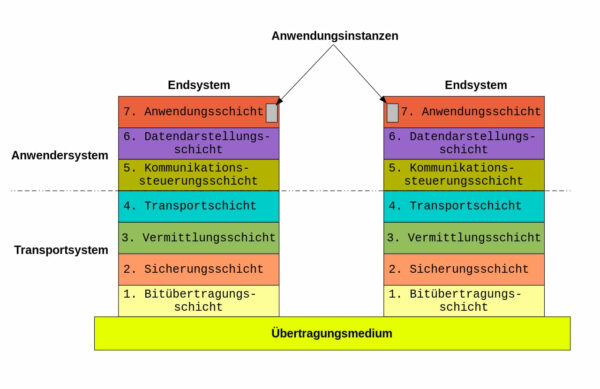
\includegraphics[width=1\linewidth]{OSI.jpg}
    \caption{Bildunterschrift} %Das steht unten drunter
    \label{fig:enter-label} %Schlüssel, um später darauf verweisen zu können
    %fig: Abbildung, tab: Tabelle; sec: Überschift (Section, Subsection); eq: Gleichung
\end{figure}


\end{document}

\printbibliography %damit das Literaturverzeichnis geprintet wird.